\documentclass{patmorin}
\listfiles
\usepackage[utf8]{inputenc}
\usepackage{amsthm,amsmath,graphicx}
\usepackage{pat}
\usepackage[letterpaper]{hyperref}
\usepackage[dvipsnames]{color}
\definecolor{linkblue}{named}{Blue}
\hypersetup{colorlinks=true, linkcolor=linkblue,  anchorcolor=linkblue,
citecolor=linkblue, filecolor=linkblue, menucolor=linkblue, pagecolor=linkblue,
urlcolor=linkblue, pdfcreator=Me, pdfproducer=Me} \setlength{\parskip}{1ex}

%\usepackage[skip=0pt]{caption}

\title{\MakeUppercase{More Turán-Type Theorems for Triangles in Convex Point Sets}\thanks{This research is partially funded by NSERC.}}
\author{Authors TBD}


\newcommand{\edgea}{\raisebox{-.1ex}{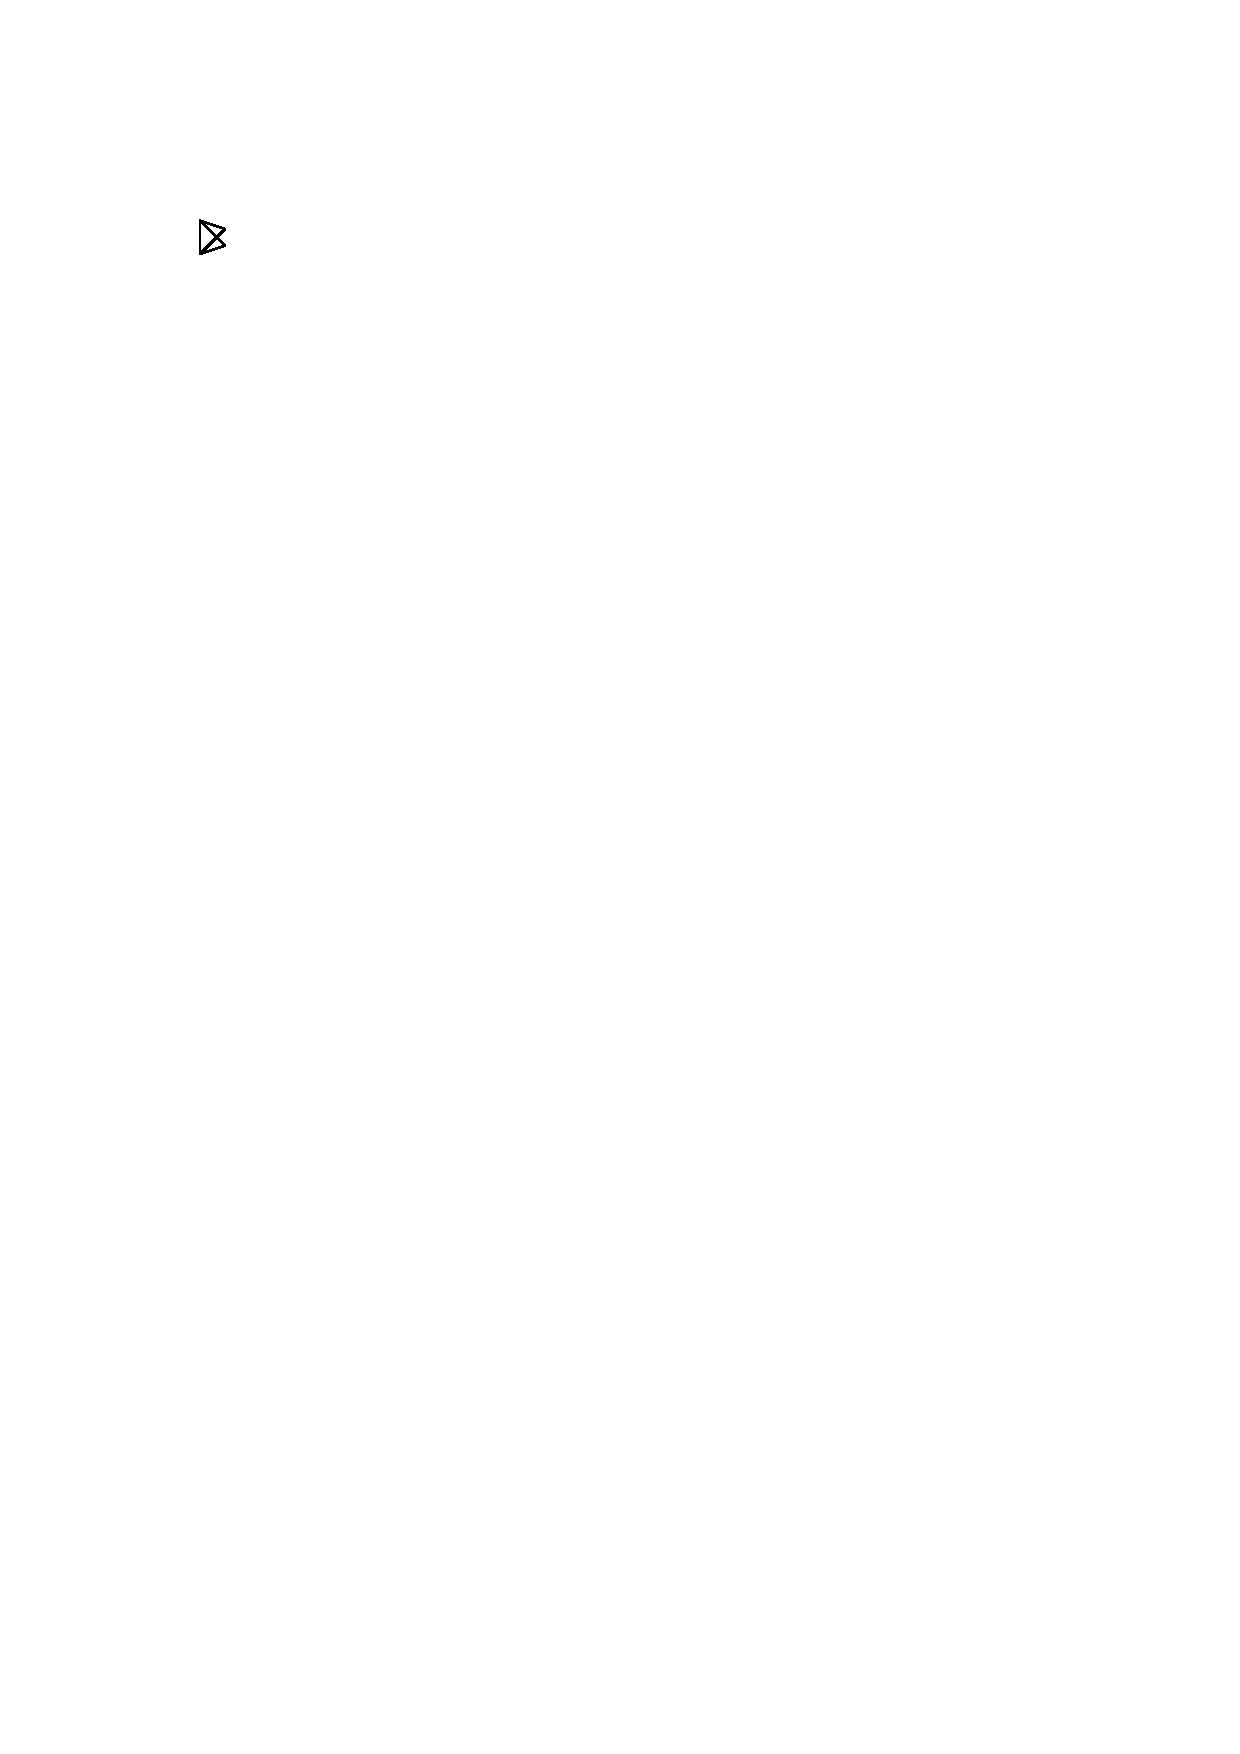
\includegraphics[height=1.6ex]{figs/triangles-edge-1}}}
\newcommand{\edgeb}{\raisebox{-.1ex}{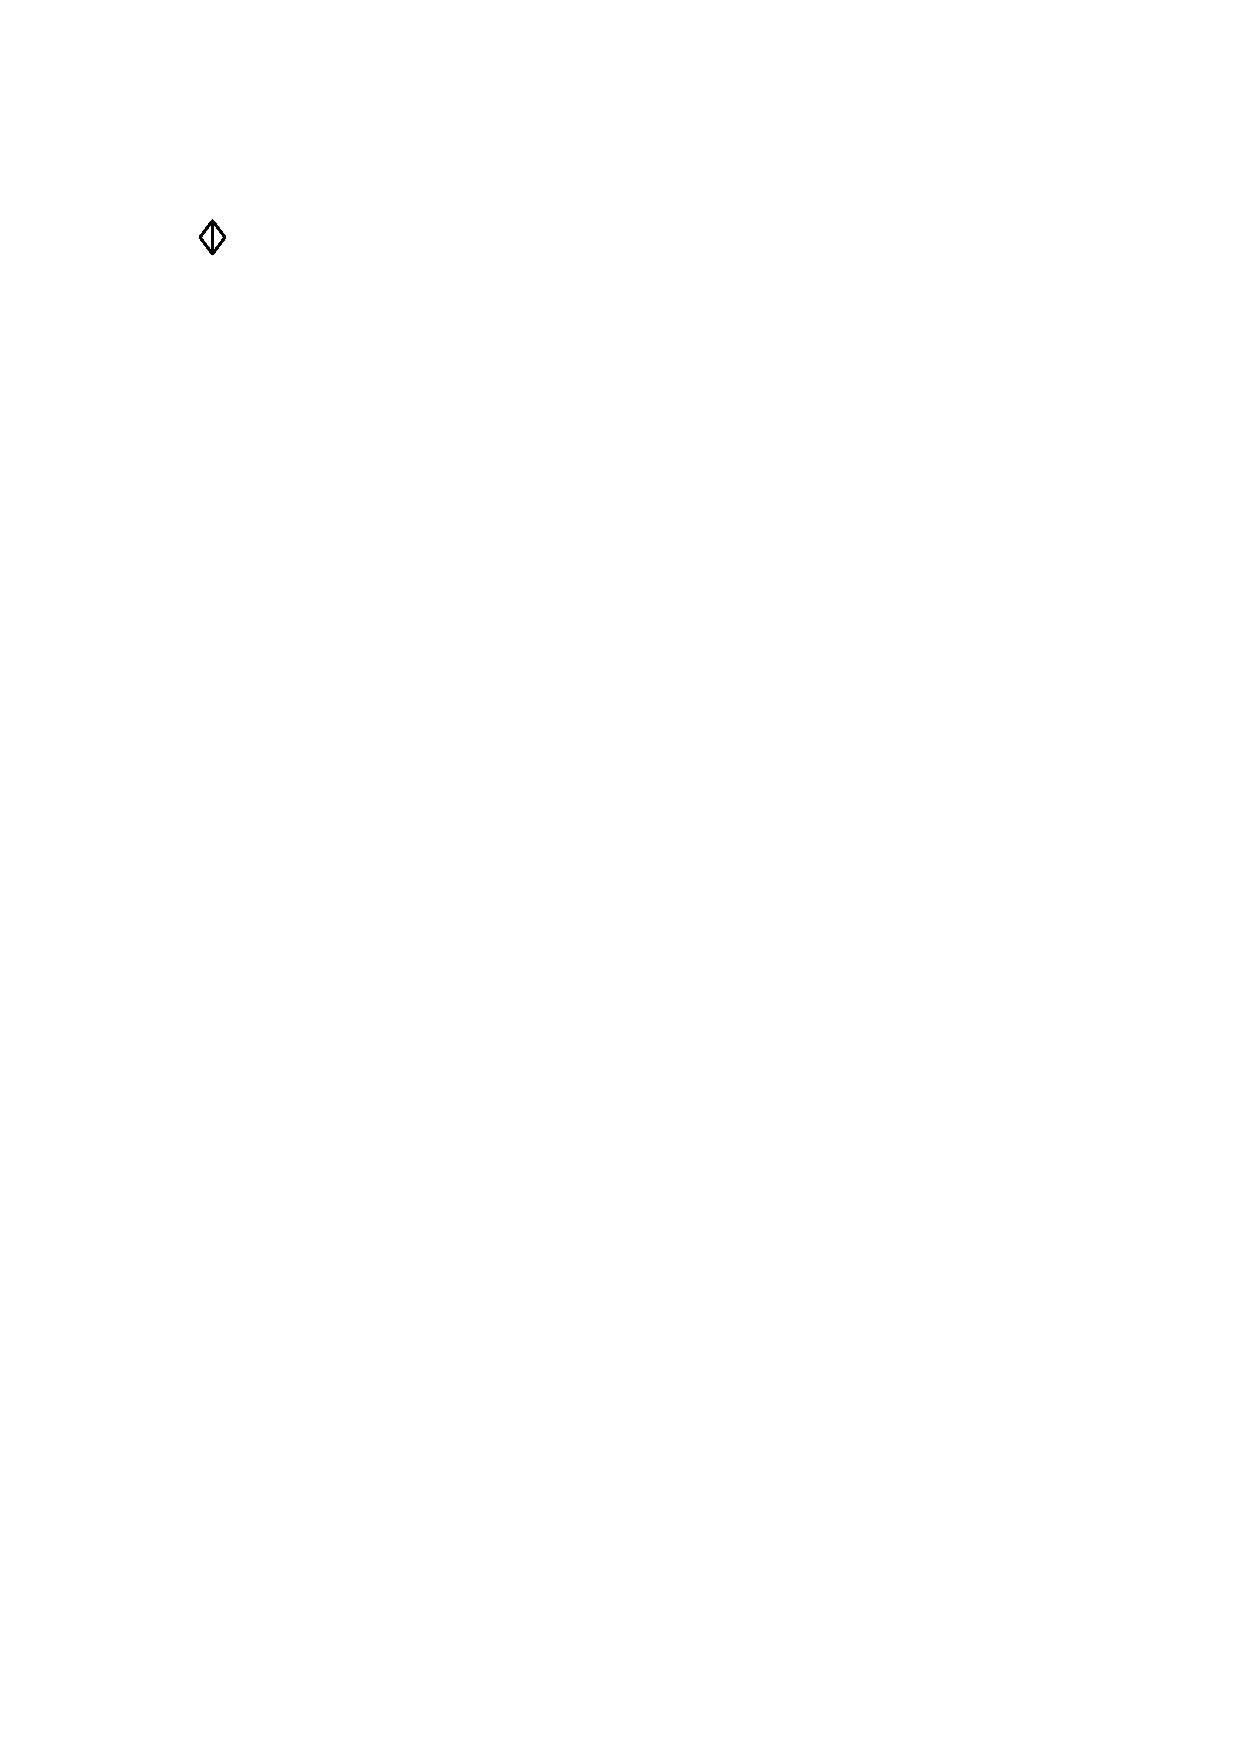
\includegraphics[height=1.6ex]{figs/triangles-edge-2}}}


\newcommand{\vertexa}{\raisebox{-.1ex}{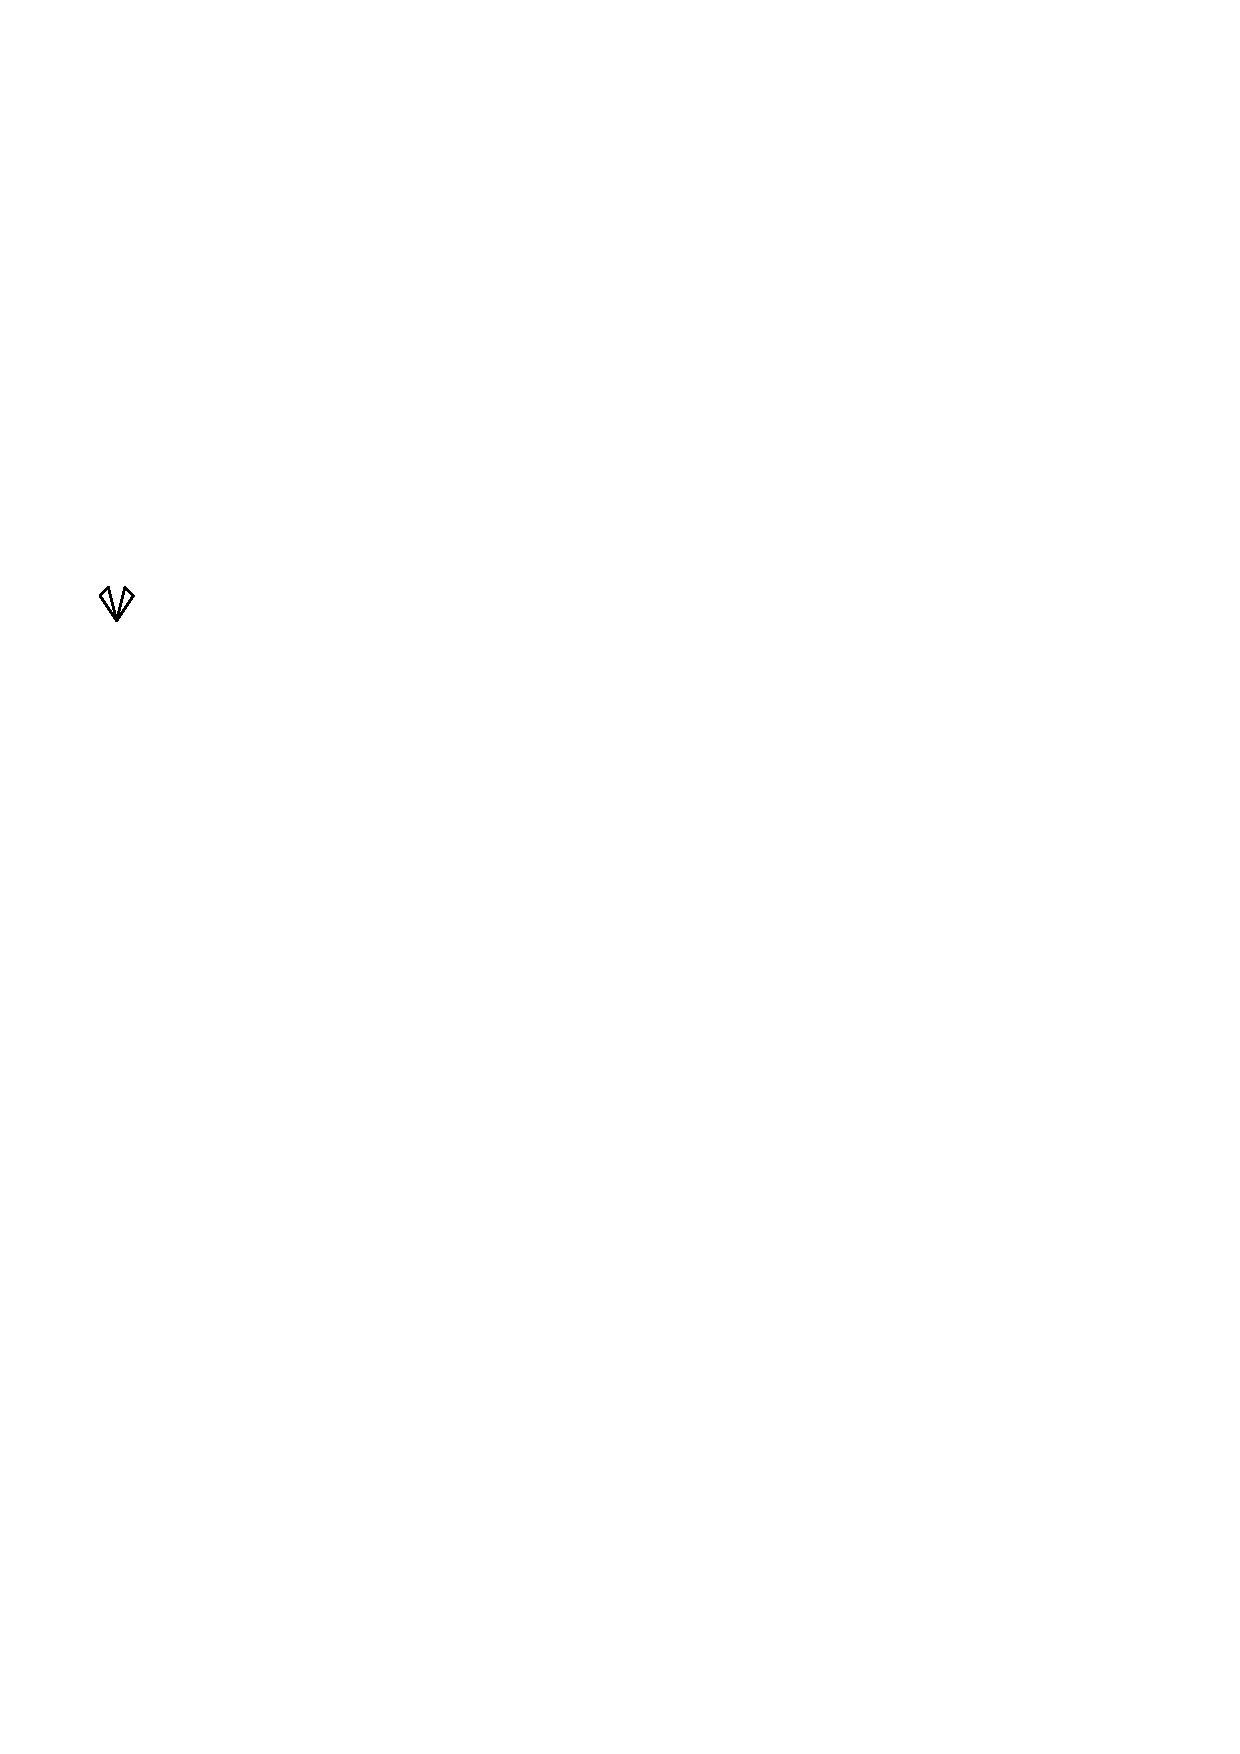
\includegraphics[height=1.6ex]{figs/triangles-vertex-1}}}
\newcommand{\vertexb}{\raisebox{-.1ex}{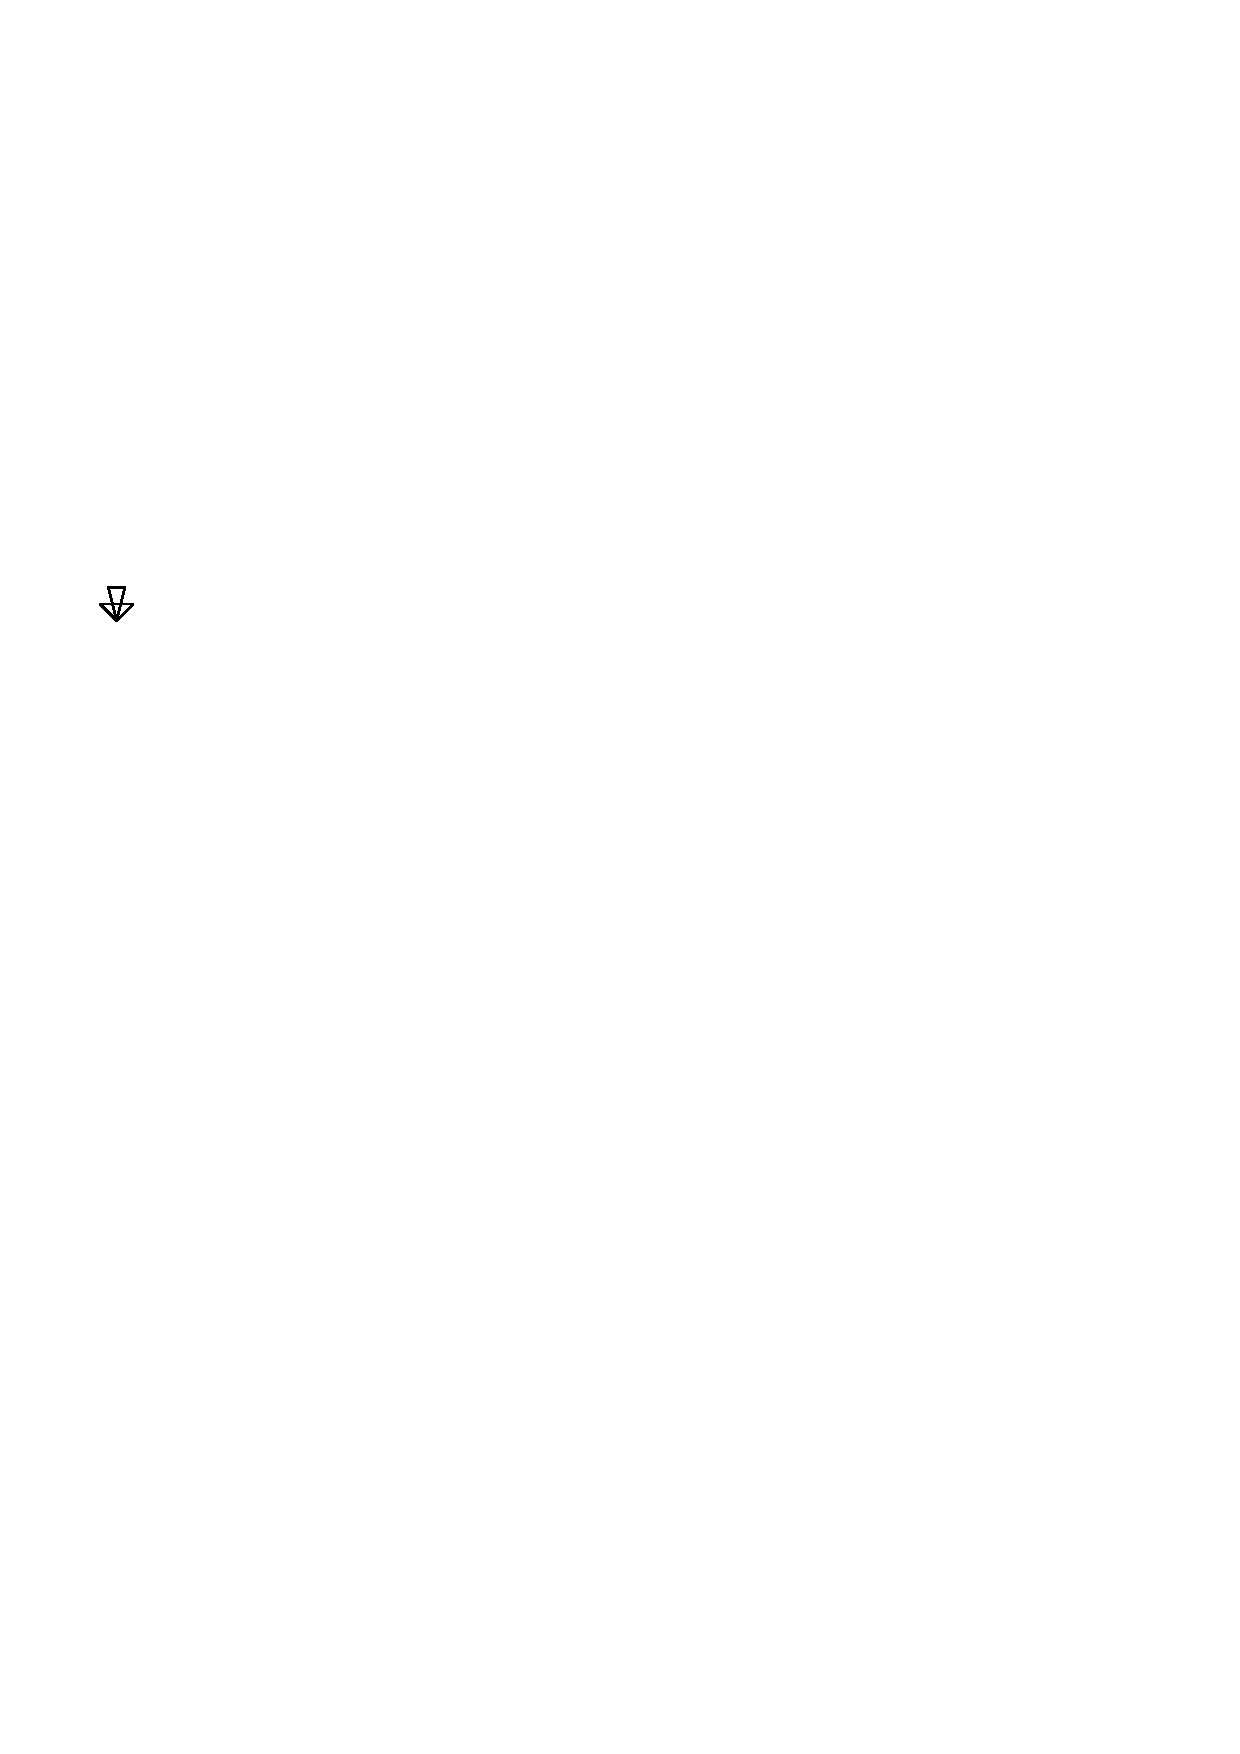
\includegraphics[height=1.6ex]{figs/triangles-vertex-2}}}
\newcommand{\vertexc}{\raisebox{-.1ex}{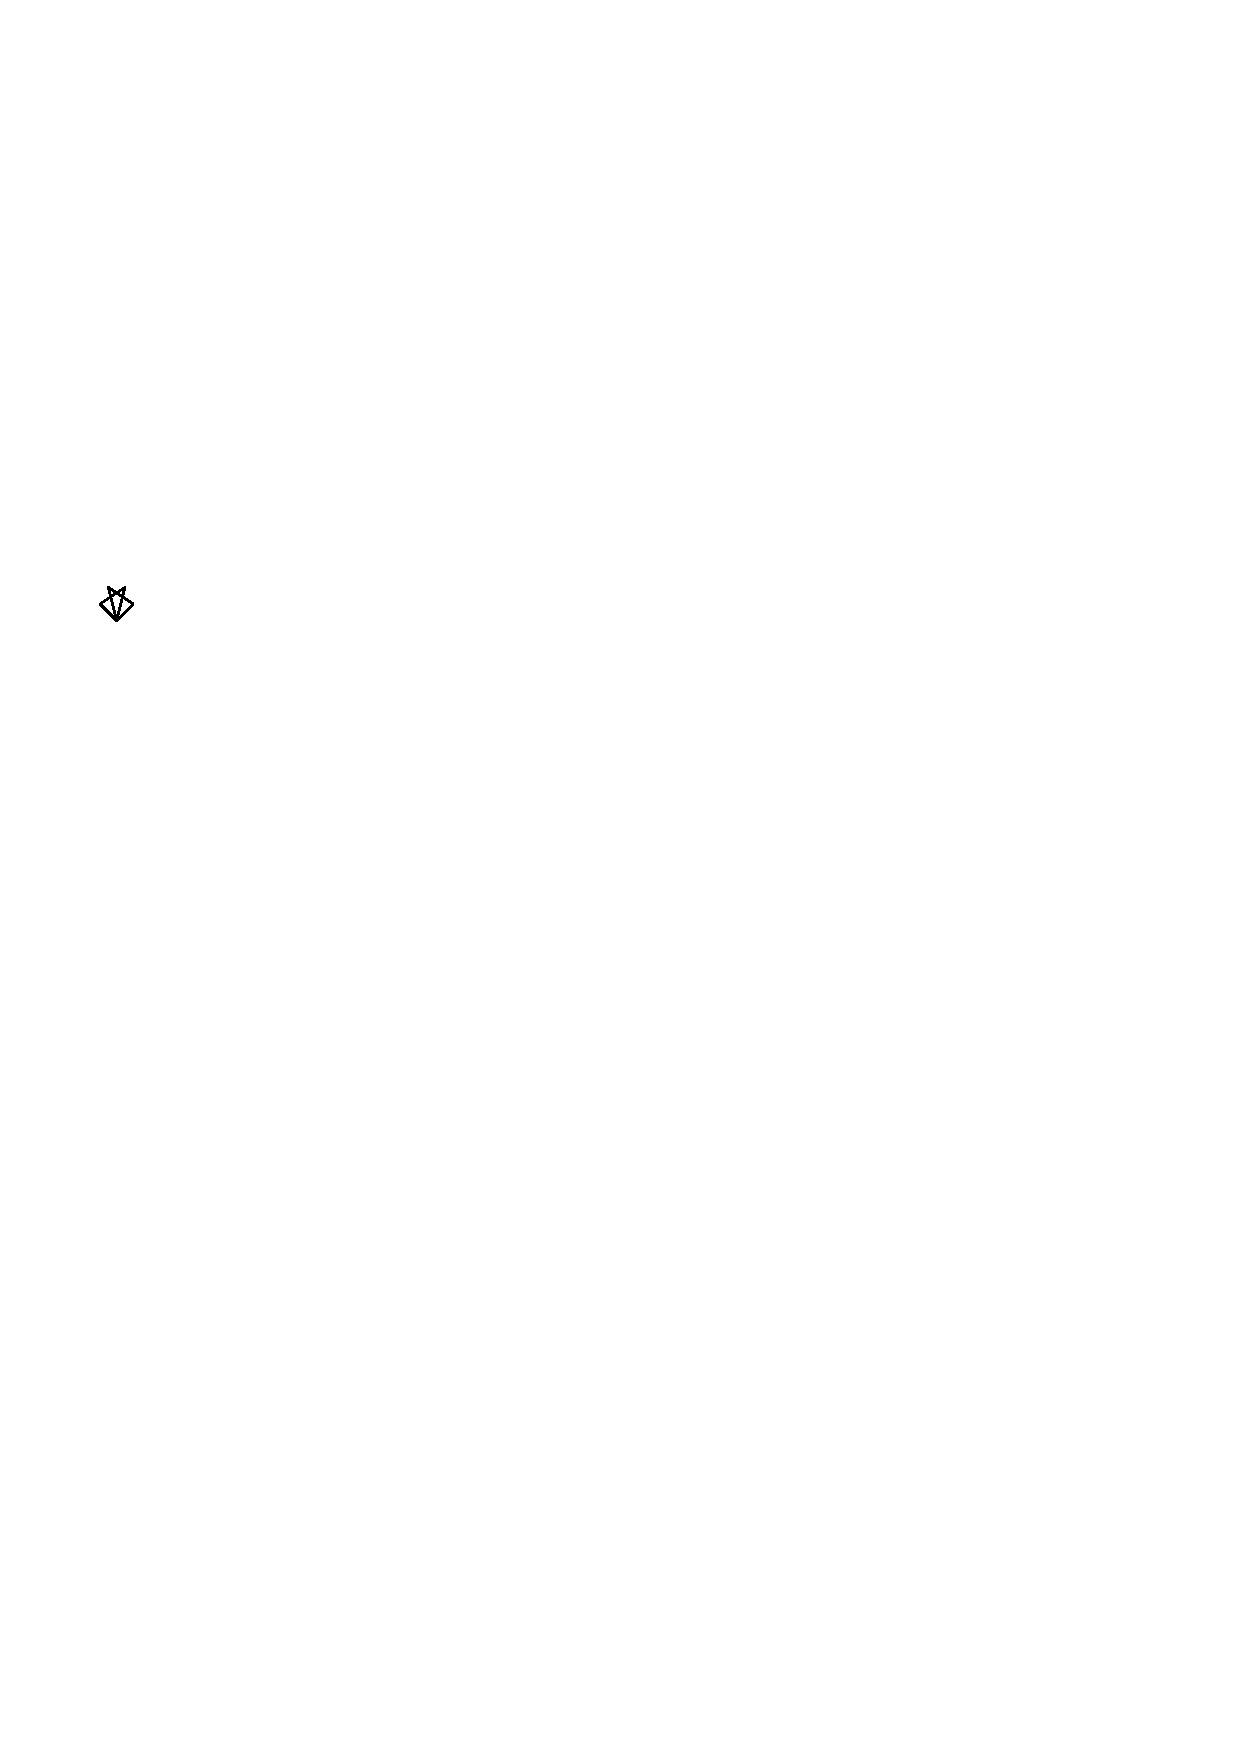
\includegraphics[height=1.6ex]{figs/triangles-vertex-3}}}

\newcommand{\disjointa}{\raisebox{-.1ex}{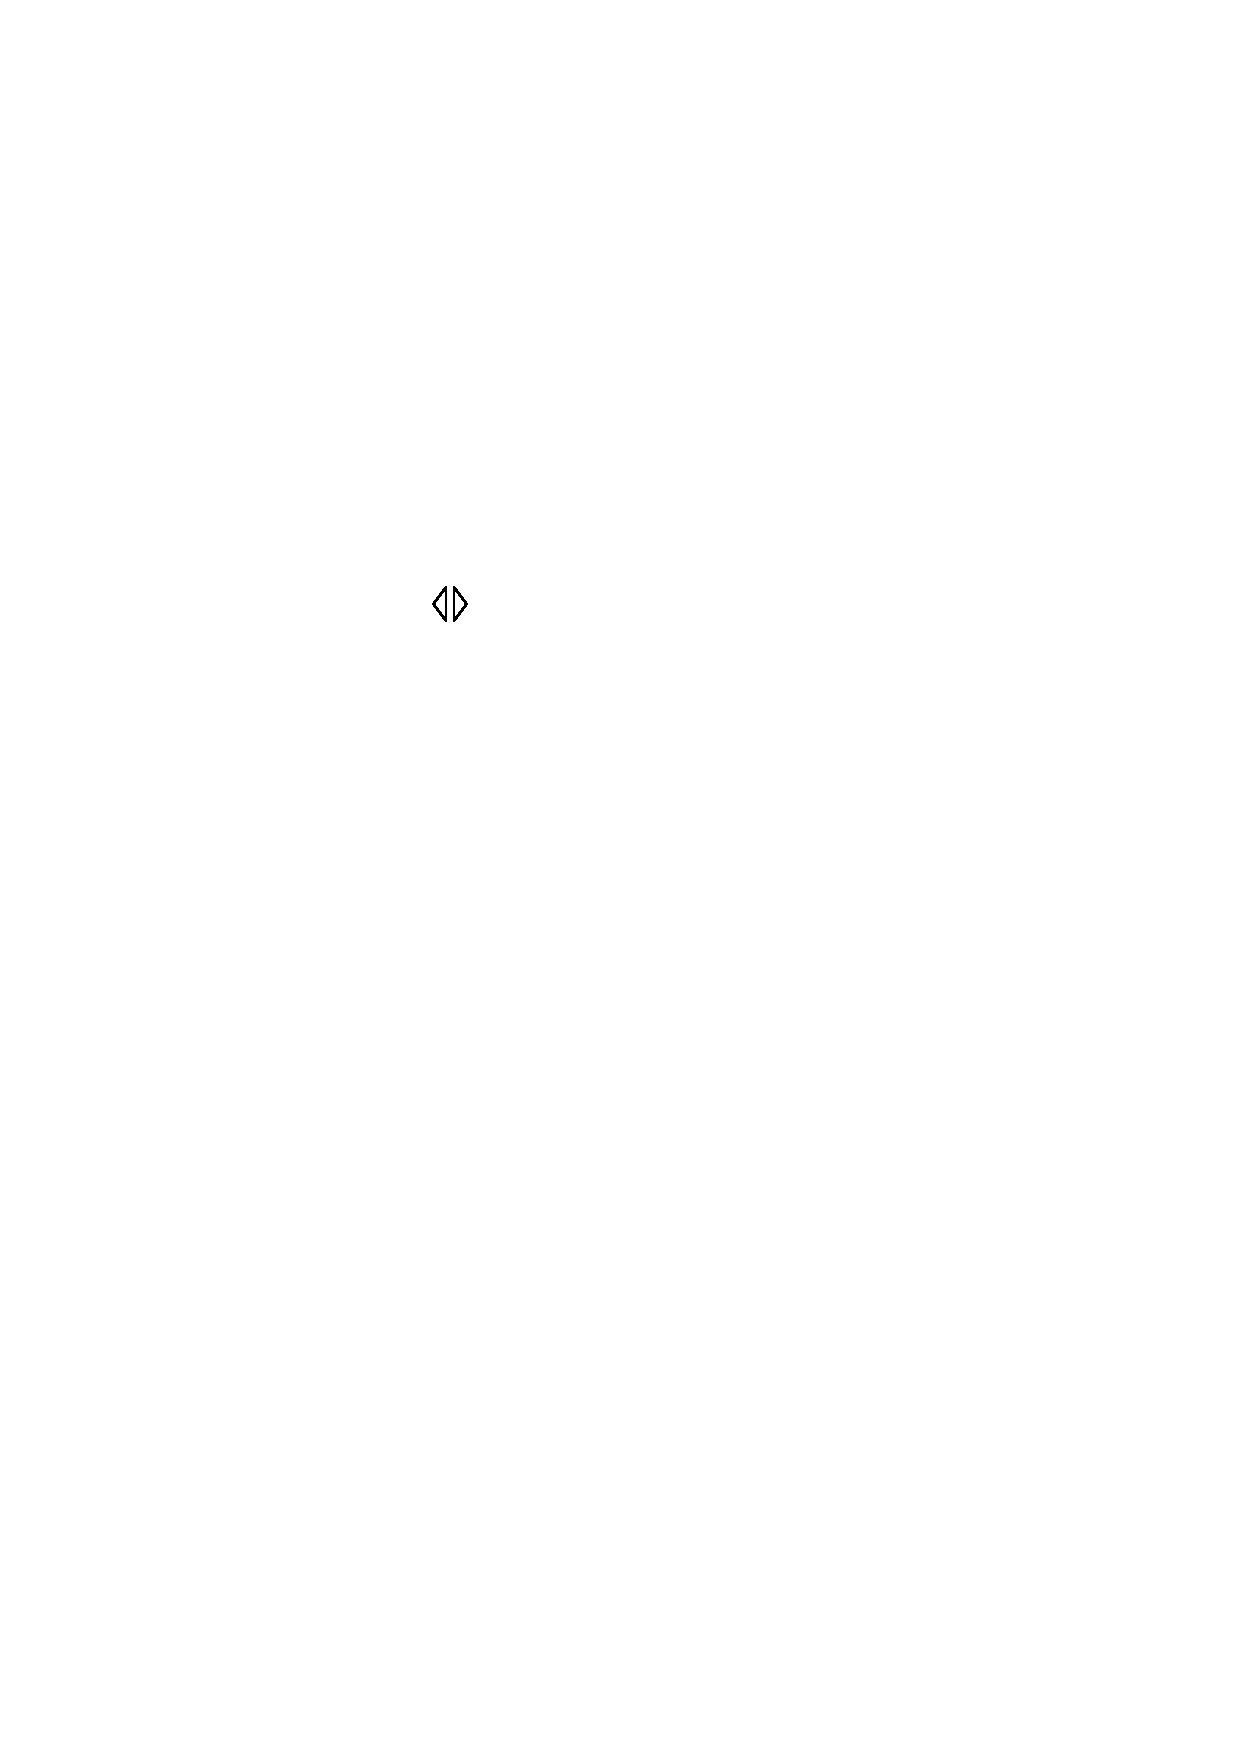
\includegraphics[height=1.6ex]{figs/triangles-disjoint-1}}}
\newcommand{\disjointb}{\raisebox{-.1ex}{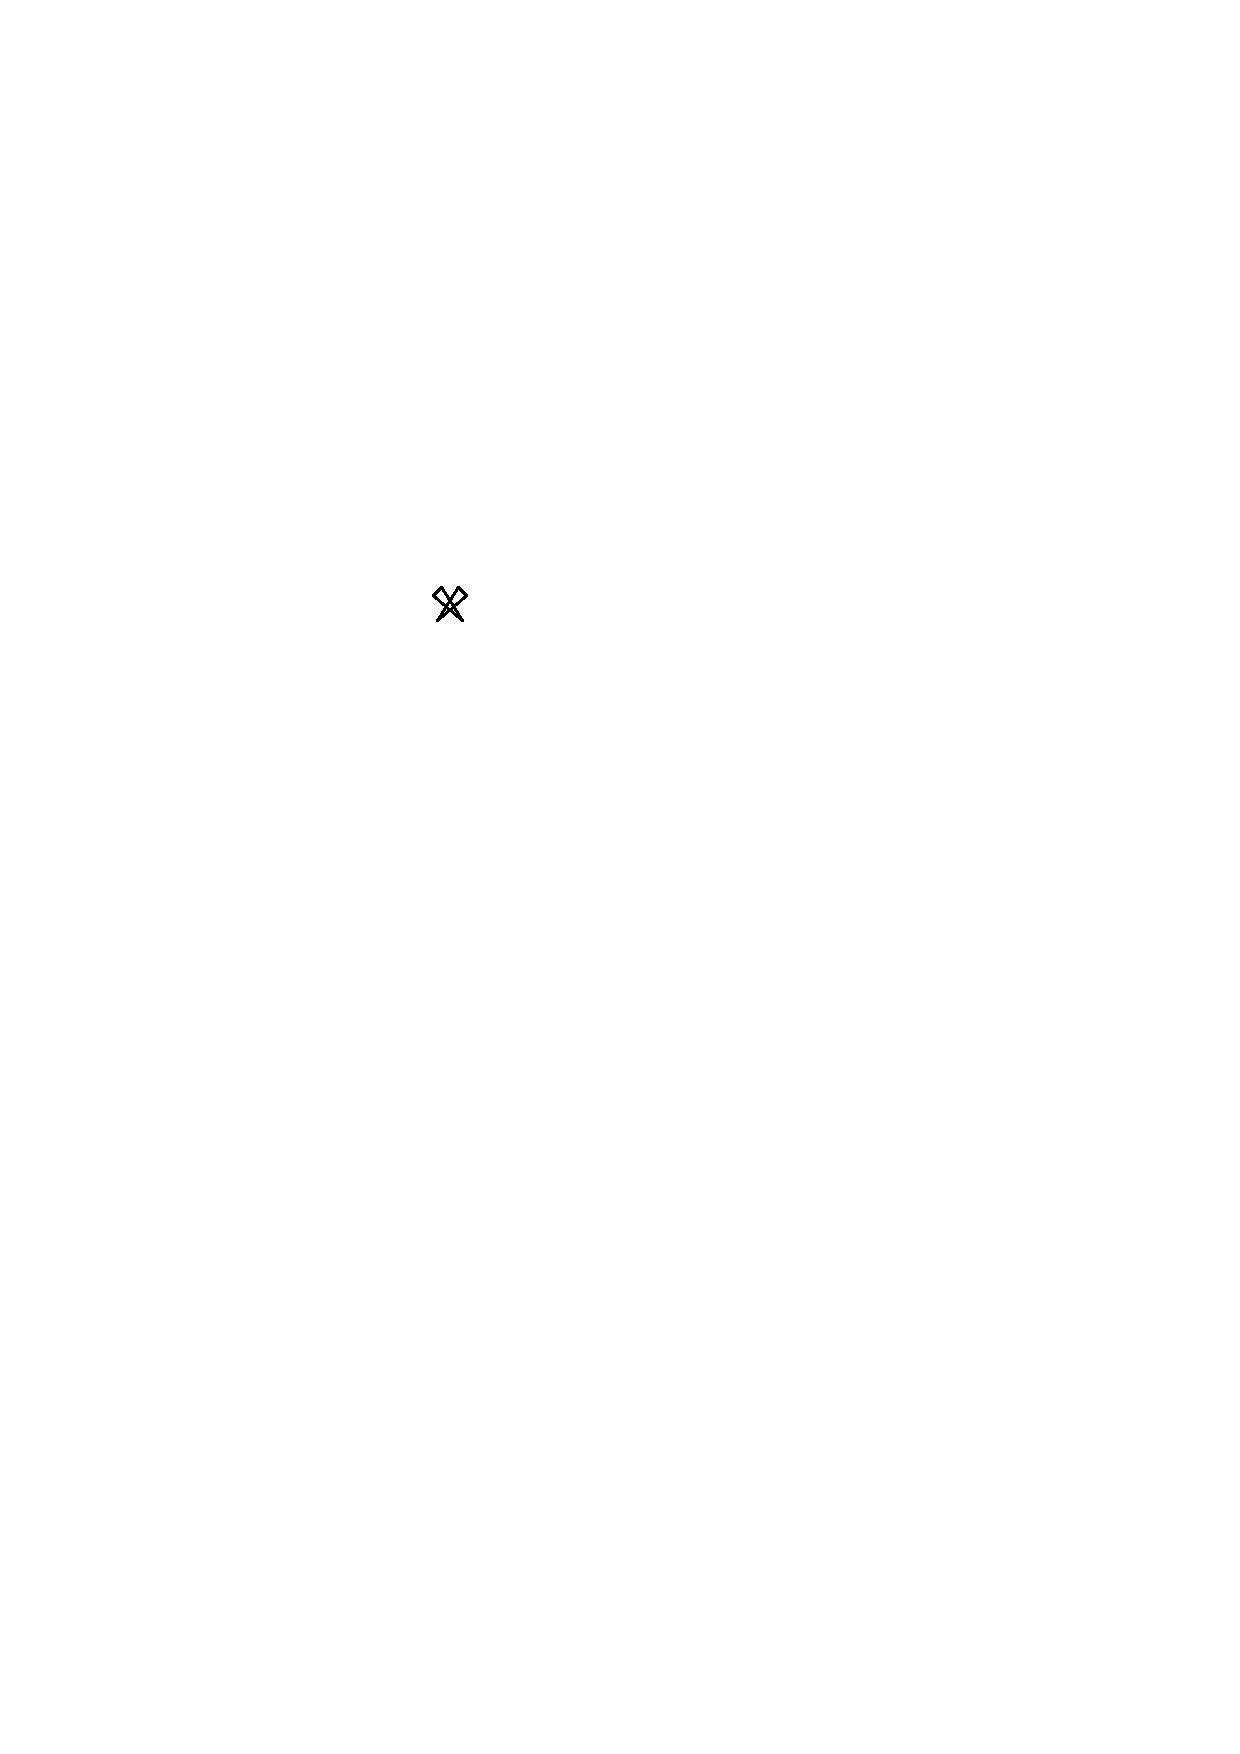
\includegraphics[height=1.6ex]{figs/triangles-disjoint-2}}}
\newcommand{\disjointc}{\raisebox{-.1ex}{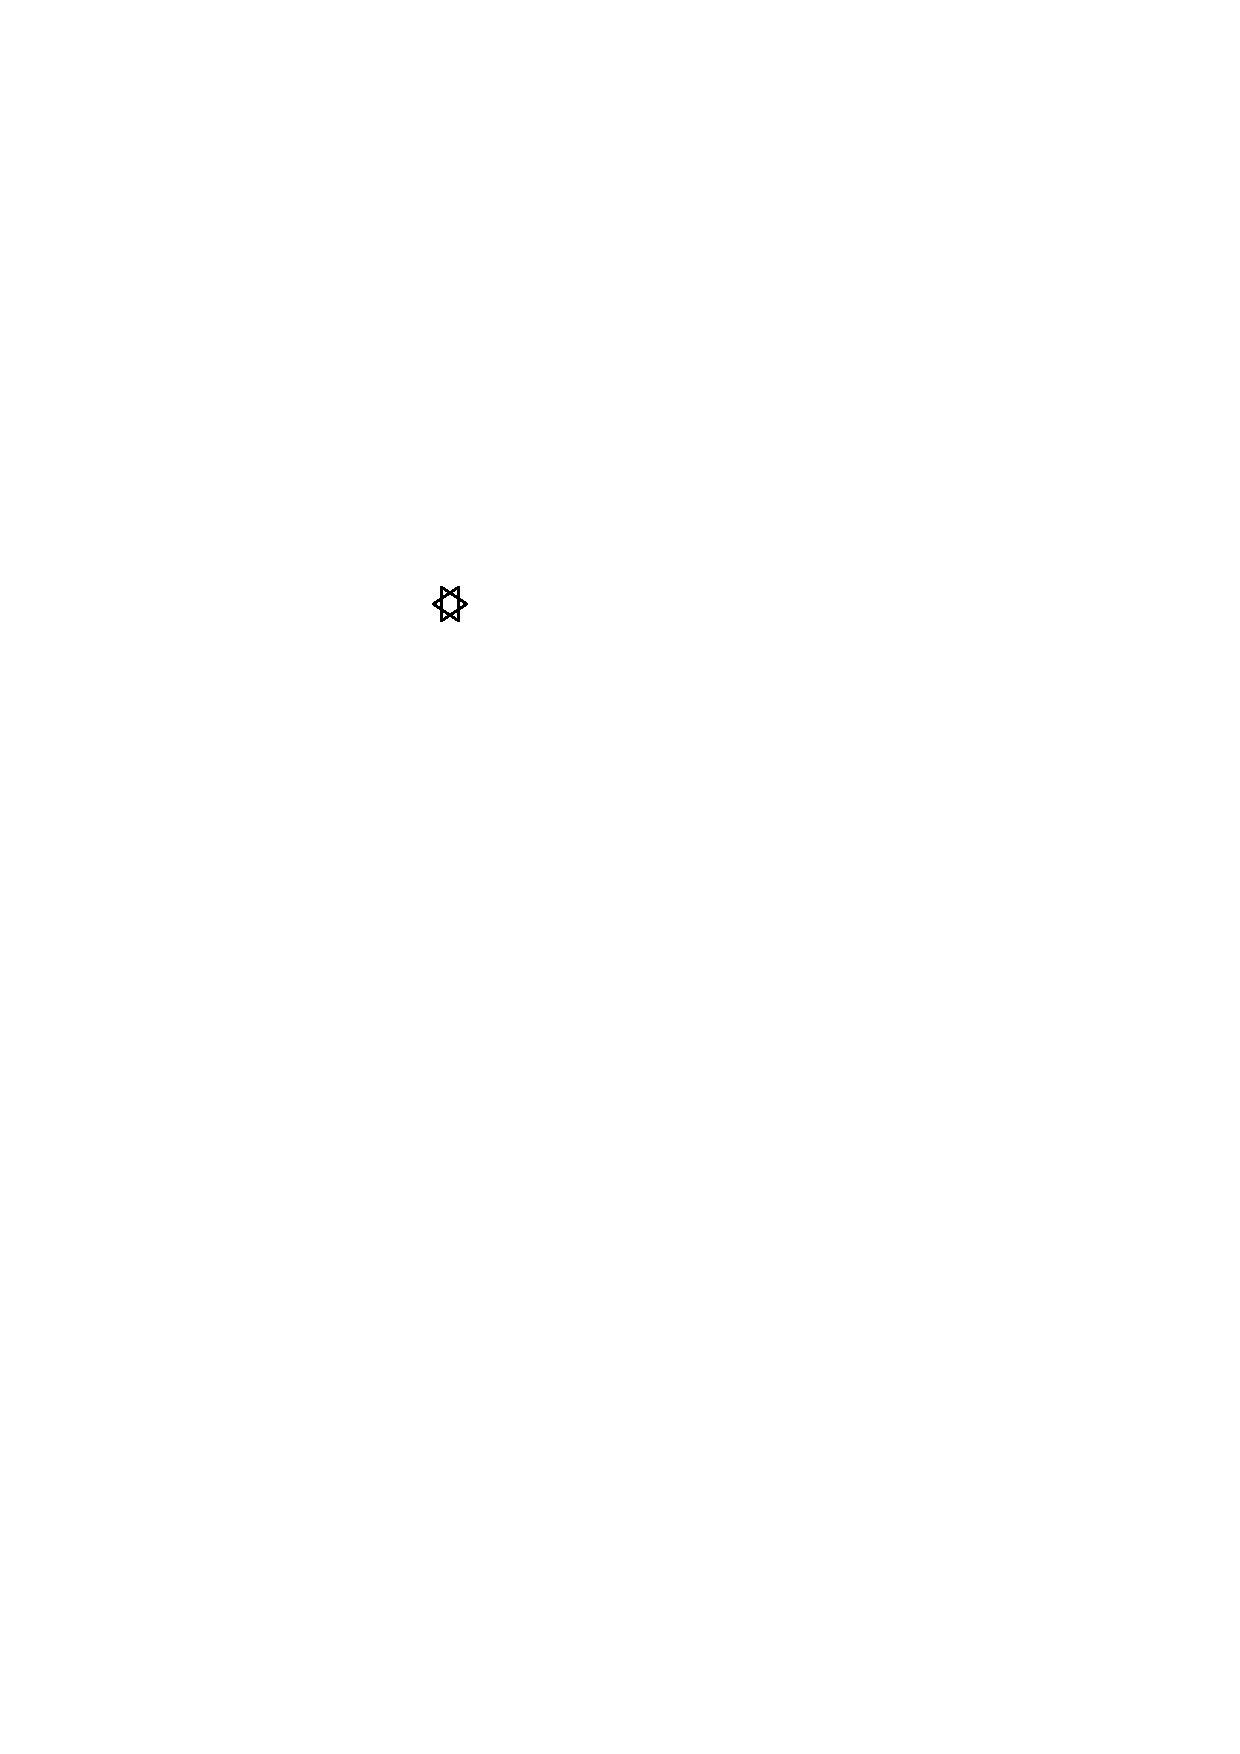
\includegraphics[height=1.6ex]{figs/triangles-disjoint-3}}}

\DeclareMathOperator{\ex}{ex}



%\usepackage{lineno}
%\linenumbers

\begin{document}
\maketitle

\begin{abstract}
  We study the following family of problems: Given a set of $n$ points
  in convex position, what is the maximum number triangles one can create
  having these points as vertices while avoiding certain \emph{forbidden
  configurations}.  As forbidden configurations we consider all 8 ways
  in which a pair of triangles in such a point set can interact.
\end{abstract}



\section{Introduction}

Let $t_1$ and $t_2$ be a pair of distinct triangles whose (4--6) vertices
are in convex position.  There are 8 combinatorially distinct ways that
these triangle can interact:  2 ways in which the triangles can share
an edge (\edgea\ and \edgeb), 3 ways in which the triangles can share a
single vertex (\vertexa, \vertexb, and \vertexc), and 3 ways in which
the triangles can have no vertices in common (\disjointa, \disjointb,
and \disjointc).

We consider the following class of problems:  Given a set, $X$,
of combinatorial configurations of pairs of triangles, what is the
largest set, $S$, of triangles one can create whose vertices are $n$
points in convex position, and such that no pair of triangles in $S$
forms a configuration in $X$.  We call the size of this set $\ex(n,X)$.
For example, 
\[
    \ex(n,\{\edgea,\vertexb,\vertexc,\disjointb,\disjointc\}) = n-2 \enspace .
\]
This is because the set
$X=\{\edgea,\vertexb,\vertexc,\disjointb,\disjointc\}$ in this case
forbids any form of crossings between the edges of triangles. Thus, the
number maximum number of triangles we can have while avoiding $X$ is the
number of triangles in a triangulation of a convex $n$-gon, i.e., $n-2$.

\begin{table}
\begin{center}
\begin{tabular}{ll}
  \hline
  $\ex(n,\{\edgeb\})\in \Theta(n^3)$ & \cite{brass:turan} \\
  $\ex(n,\{\edgea\})\in \Theta(n^2)$ & \cite{brass:turan} \\
  \hline
  $\ex(n,\{\vertexa\})\in \Theta(n^3)$ & \cite{brass:turan} \\
  $\ex(n,\{\vertexb\})\in \Theta(n^2)$ & \cite{brass:turan} \\
  $\ex(n,\{\vertexc\})\in \Theta(n^2)$ & \cite{brass:turan} \\
  \hline
  $\ex(n,\{\disjointa\})\in \Theta(n^3)$ & \cite{brass:turan} \\
  $\ex(n,\{\disjointb\})\in \Theta(n^2)$ & \cite{brass:turan} \\
  $\ex(n,\{\disjointc\})\in \Theta(n^2)$ & \cite{brass:turan} \\
  \hline
  $\ex(n,\{\vertexa,\vertexb\})\in \Theta(n^2)$ & \cite{brass:turan} \\
  $\ex(n,\{\vertexb,\vertexc\})\in \Theta(n^2)$ & \cite{brass:turan} \\
  $\ex(n,\{\vertexa,\vertexc\})\in \Theta(n^2)$ & \cite{brass:turan} \\
  \hline
  $\ex(n,\{\disjointa,\disjointb,\vertexa,\vertexb\}) = n$ & \cite{brass.rote.ea:triangles} \\
  \hline
  $\ex(n,\{\edgea,\vertexb\}) \in \Omega(n^{3/2})\cap O(n^2)$ & here \\
  $\ex(n,\{\edgea,\vertexb,\vertexc\}) \in \Theta(n)$ & \thmref{blech} \\
  $\ex(n,X\cup\{\edgeb\})\in \Theta(\ex(n,X))$ & \lemref{xcup} \\
  \end{tabular}
\end{center}
\caption{Known and new results on $\ex(n,X)$ for different sets $X$.}
\end{table}


\section{Some Easy Results}


The following lemma shows that including the $\edgea$ confguration in
the set $X$ of forbidden configurations has no effect on the asymptotics
of $\ex(n,X)$.

\begin{lem}\lemlabel{xcup}
   For any $X$, $\ex(n,X\cup\{\edgeb\}) \ge \ex(n,X)/8$.
\end{lem}

\begin{proof}
  Let $S$ be a set of triangles that achieves $\ex(n,X)$. For each pair
  of vertices $u$ and $w$ independently and uniformly choose a direction
  $\overrightarrow{uw}$ or $\overleftarrow{uw}$.  We then obtain a set
  $S'\subseteq S$ by removing any triangle that has a directed edge for
  which the triangle is to the left of the edge.  Observe that the set
  $S'$ does not contain a $\edgeb$ configuration.

  For any particular triangle $t\in S$, the probability that $t\in S'$
  is exactly $1/8$ since each of $t$'s three edges much be directed
  clockwise and edge directions are chosen independently.  By linearity of
  expectation, $\E[|S'|]=|S|/8=\ex(n,X)/8$.  We conclude therefore that
  there exists some subset $S''\subseteq S$ of size least $\ex(n,X)/8$
  that does not contain a $\edgeb$ configuration.  The set $S''$ proves
  that $\ex(n,X\cup\{\edgeb\}) \ge \ex(n,X)/8$.
\end{proof}

From this point onward, we will frequently include \edgeb\ in sets of
forbidden configurations when proving upper bounds.  By \lemref{xcup}
any upper bound we prove this way holds (within a factor of 8) without
including \edgeb.

It will be helpful to consider an top/bottom variant of $\ex(n,X)$ that
is defined as follows.  Partition the vertices of a convex $n$-gon using a
horizontal line into a \emph{top half} of size $\lfloor n/2\rfloor$ and
a \emph{bottom half} of size $\lceil n/2\rceil$.  We define $\ex'(n,X)$
analogously to $\ex(n,X)$ except that we only count triangles have one
vertex in the bottom half and one vertex in the top half.

The following lemma helps us use divide-and-conquer to prove upper bounds:

\begin{lem}\lemlabel{top-bottom}
  If $\ex'(n,X)\in O(n^c)$, then
\[
   \ex(n,X)\in 
      \begin{cases} 
          O(n^c)     & \text{if $c>1$} \\
          O(n\log n) & \text{if $c=1$}
      \end{cases}
\]
\end{lem}

\begin{thm}\thmlabel{blech}
  $\ex(n,\{\edgea,\vertexb,\vertexc\}) \in \Omega(n)\cap O(n\log n)$.
\end{thm}

\begin{proof}
  The $\Omega(n)$ lower bound is achievable by many constructions including,
  for example, any triangulation of a convex $n$-gon.

  To prove the $O(n\log n)$ upper bound, it suffices---by
  Lemmas~\ref{lem:xcup} and \ref{lem:top-bottom}---to show that
  $\ex'(n,\{\edgea,\vertexb,\vertexc,\edgeb\})\in O(n)$.
\end{proof}





\bibliographystyle{plainurl}
\bibliography{turan}

\end{document}


